\documentclass{beamer}
\usepackage{fontspec} \usepackage{xunicode} \usepackage{xltxtra} \usepackage{xecyr} \usepackage{hyperref}
\usepackage{ragged2e} \usepackage{tabularx} \setmainfont[Mapping=tex-text]{DejaVu Serif}
\setsansfont[Mapping=tex-text]{DejaVu Sans} \setmonofont[Mapping=tex-text]{DejaVu Sans Mono}
\usepackage{polyglossia} \setdefaultlanguage{russian} \usepackage{graphicx} \usepackage{color} \usepackage{listings}

\renewcommand*{\inserttotalframenumber}{\pageref{lastframe}}
\beamertemplatenavigationsymbolsempty

\lstdefinestyle{mycode}{
  belowcaptionskip=1\baselineskip,
  breaklines=true,
  xleftmargin=\parindent,
  showstringspaces=false,
  basicstyle=\footnotesize\ttfamily,
  keywordstyle=\bfseries,
  commentstyle=\itshape\color{gray!40!black},
  stringstyle=\color{red},
  numbers=left,
  numbersep=5pt,
  numberstyle=\tiny\color{gray},
}

\addtobeamertemplate{navigation symbols}{}{
    \usebeamerfont{footline}%
    \usebeamercolor[fg]{footline}%
    \hspace{1em}%
     {\small\color{black}{\insertframenumber/\inserttotalframenumber}} 
}

\defbeamertemplate*{title page}{customized}[1][]{

  \begin{center}
  \bigskip
  \usebeamerfont{title}\inserttitle\par
  \usebeamerfont{subtitle}\usebeamercolor[fg]{subtitle}\insertsubtitle\par
  \bigskip
  \color{black}{\usebeamerfont{author}\insertauthor}\par
  \bigskip
  \usebeamerfont{institute}\insertinstitute\par
  \bigskip
  {\scriptsize\usebeamerfont{date}\insertdate}\par
  \usebeamercolor[fg]{titlegraphic}\inserttitlegraphic
  \end{center}
}


\lstset{escapechar=@,style=mycode}
\setbeamerfont{frametitle}{size=\LARGE}

\title{ Матчинг отзывов и организаций в Яндексе }
%\subtitle{или как всё закодить в декабре, переписать в феврале и поседеть в апреле}
\institute{Яндекс.Отзывы}
\author{{\small Антон Алексеев, CSC\\anton.m.alexeyev@yandex.ru\\}}
\date{5 июня 2014 г.}

\begin{document}

%1. Титульный слайд
% Генерируется автоматичсеки

{
\setbeamertemplate{navigation symbols}{} 
\setbeamertemplate{footline}{} 
\frame{\titlepage}
}
%2. Структура доклада

\begin{frame}\frametitle{План}
    \begin{enumerate}
        \item Что такое Яндекс.Отзывы
        \item Постановка задачи
        \item Старый матчинг
        \item Новый матчинг
        \item Результаты и выводы
    \end{enumerate}
\end{frame}


\begin{frame}\frametitle{Яндекс.Отзывы}

\begin{itemize}
\item Яндекс --- это не только {\color{red}Я}ndex.ru
\item Много сервисов с отзывами
\item Единая платформа для хранения, обработки и предоставления доступа~к
\end{itemize}

[Здесь должен быть скриншот смешного отзыва]

\end{frame}


\begin{frame} \frametitle{Какие бывают отзывы?}
	По типу источника
	\begin{itemize}
	\item Свои (user generated content)
	\item Партнёрские
		\begin{itemize}
		\item Микроразметка \item Фиды \item Спецроботы
		\end{itemize}
	\end{itemize}
        По типу объекта
	\begin{itemize}
	\item На организации \item На приложения \item На автомобили \item etc.
	\end{itemize}
\end{frame}

\begin{frame} \frametitle{Партнёрские отзывы на организации}
	То, что получаем от партнёров
	\begin{itemize}
	\item Собственно отзыв
		\begin{itemize}
		\item текст \item ссылка \item рейтинг  \item etc.
		\end{itemize}
	\item Организация
		\begin{itemize}
		\item наименование \item ссылка	\item адрес \item телефон \item категория?  \item etc.
		\end{itemize}
	\item Бессмертный автор
		\begin{itemize}
		\item имя \item etc.
		\end{itemize}
	\end{itemize}
\end{frame}


\begin{frame}\frametitle{Задача}
	\begin{itemize}
		\item Каждому отзыву умеем сопоставлять организацию из Яндекс.Справочника
		\item Много, много жалоб на матчинг от владельцев организаций, партнёров и пользователей
		\item<2> \textbf{Повысить точность сопоставления, не убивая полноту}
	\end{itemize}
\end{frame}

\begin{frame}\frametitle{Отступление}
\begin{figure}[ht]
\begin{center}
%\includegraphics[height=3in]{matching.png}
\end{center}
\end{figure}
$$Recall_{total} = \frac{Right + Wrong}{Right + Wrong + Skipped + Trash}$$
$$Precision_{important} = \frac{Right}{Wrong}$$
$$Recall_{important} = \frac{Right}{Right + Skipped}$$
\end{frame}

\begin{frame}\frametitle{Как всё устроено}
\begin{figure}[ht]
\begin{center}
%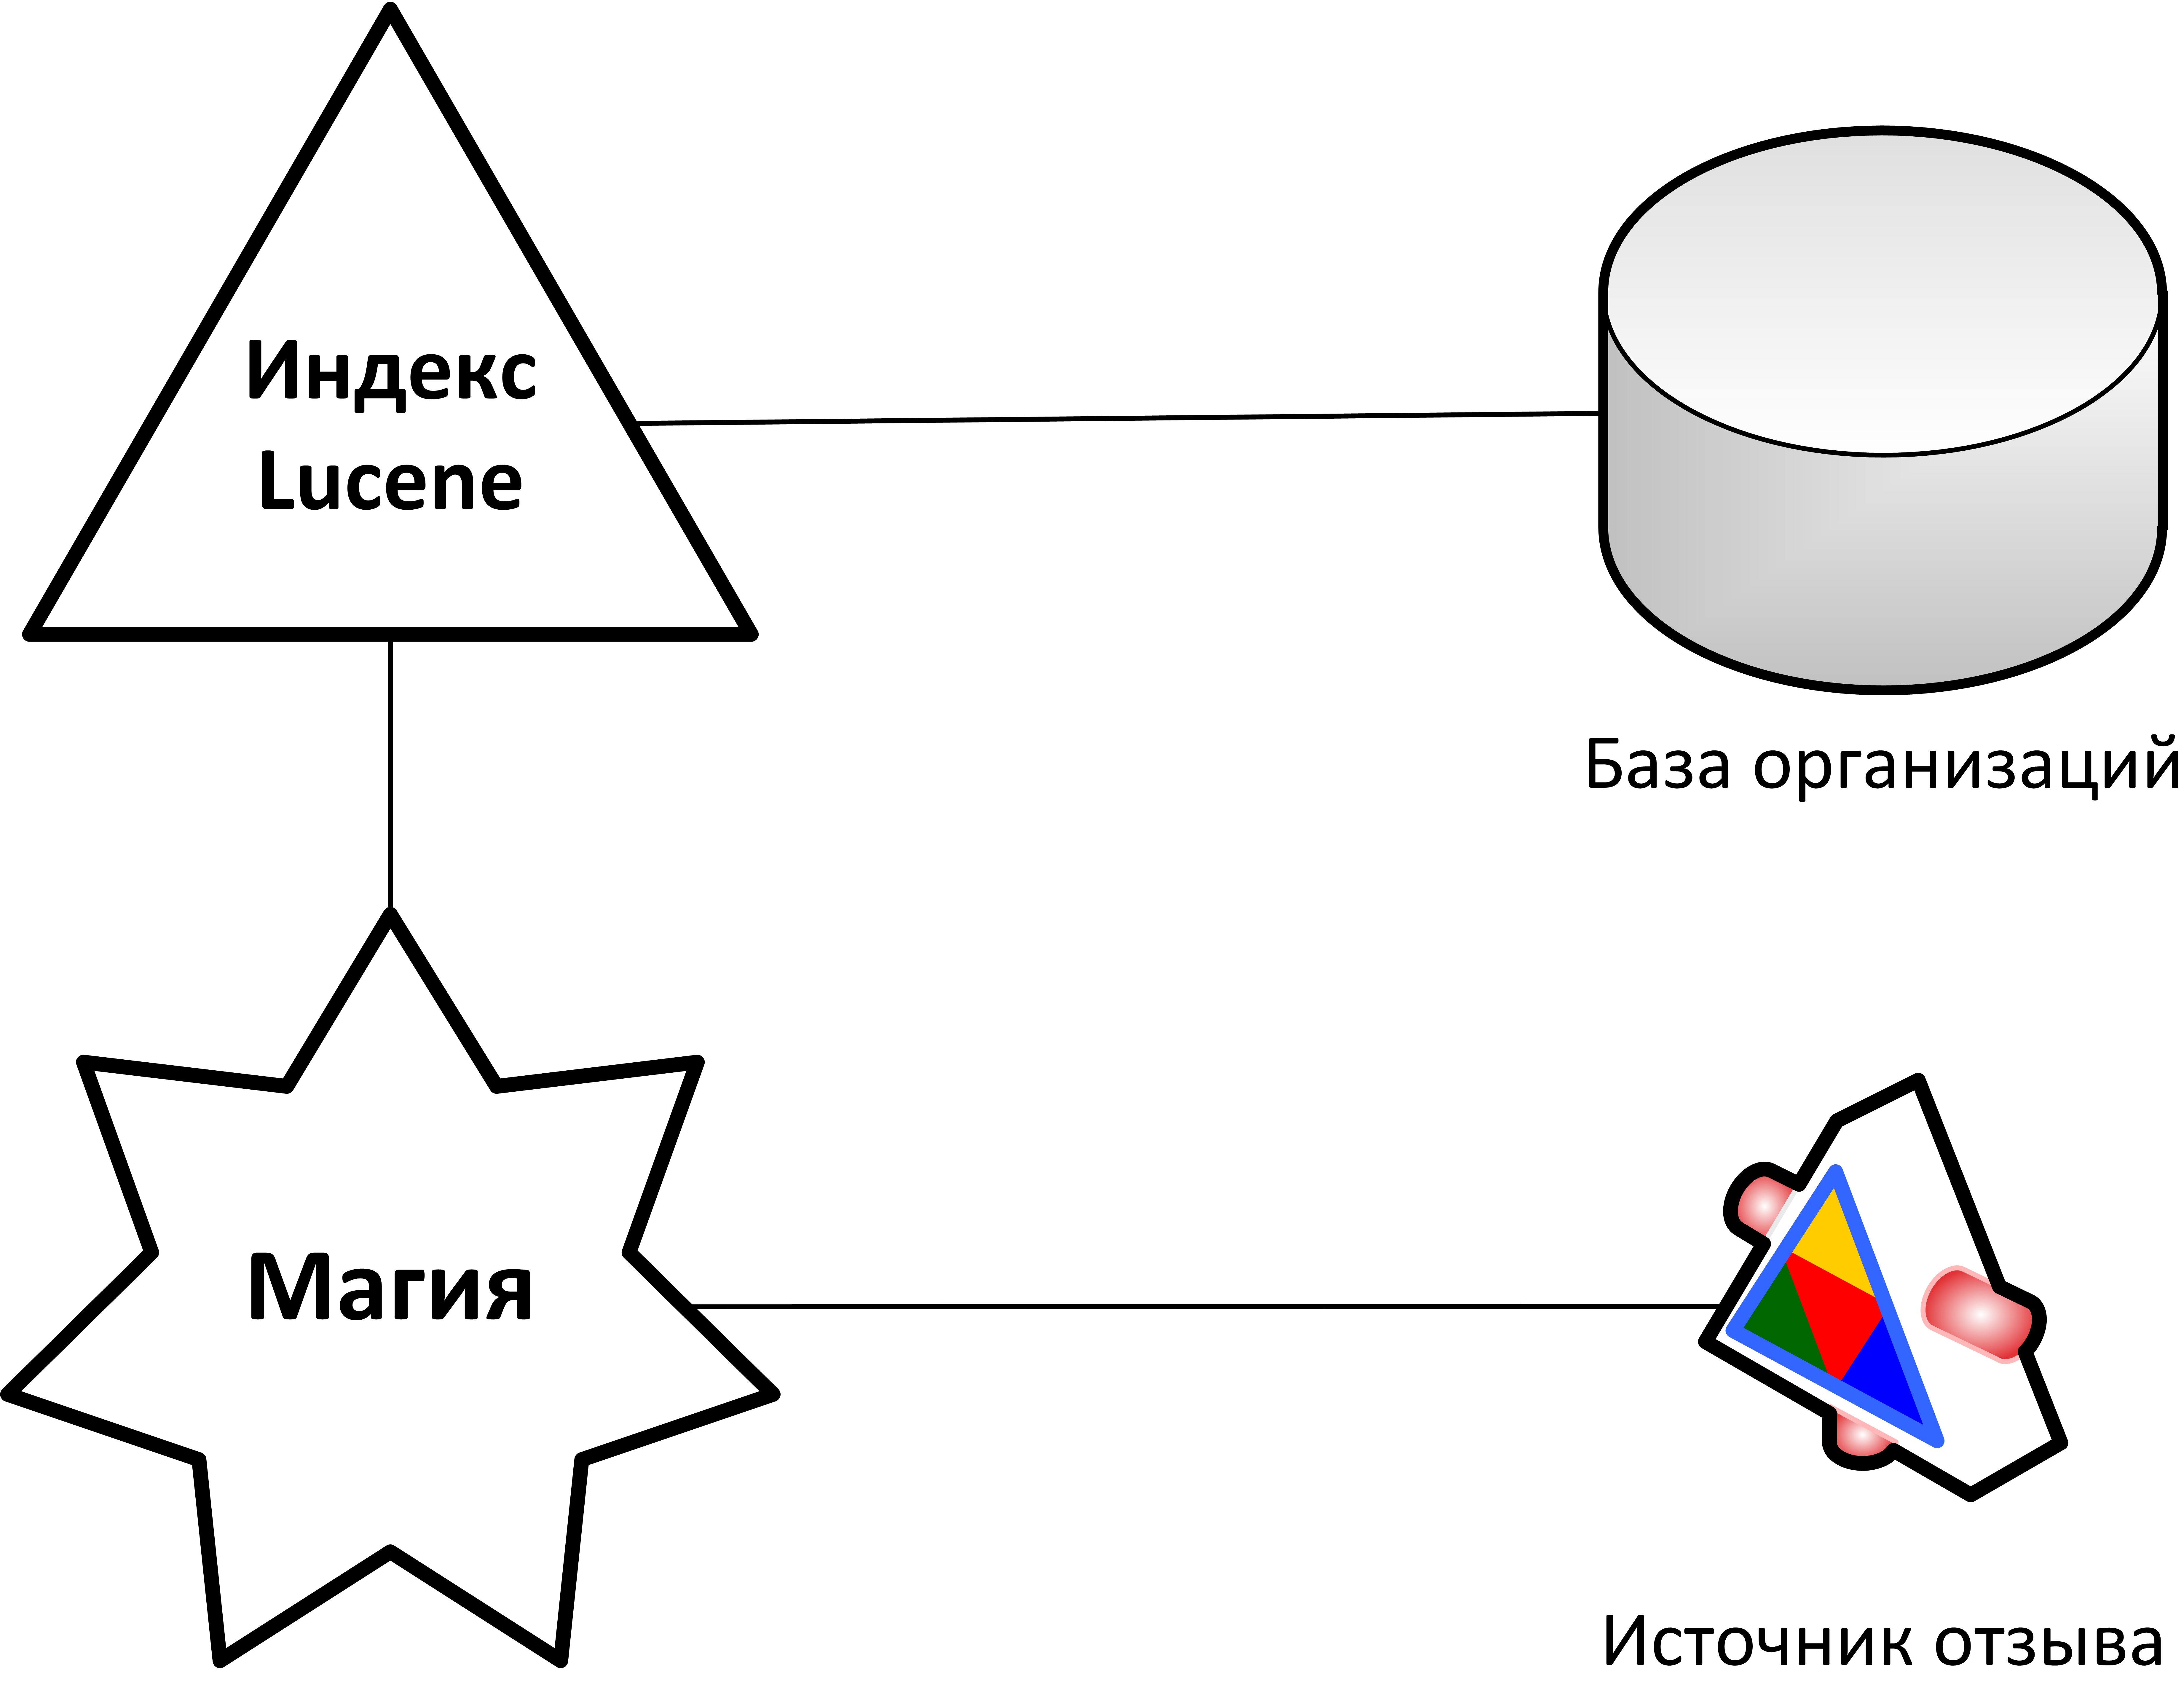
\includegraphics[height=3in]{magic.png}
\end{center}
\end{figure}
\end{frame}

\begin{frame}\frametitle{Старая магия}
{\small
	\begin{tabularx}{\textwidth}{XlX}
	  "+7 (812) 2-12-85-0-6" & $\rightarrow$  & [phone:60581222187] \newline \\
	  "Санкт-Петебург,\newline Столярный пер., 5." & $\rightarrow$ & [address:санкт-петербург \newline address:столярный \newline address:пер address:5] \newline \\
	  "Бабушкин комод" & $\rightarrow$  & [name:бабушкин name:комод] \\
	\end{tabularx}
}
\textbf{Фильтрующий запрос:} должны встречаться хотя бы один терм из адреса и один терм из названия.\\
Для \textbf{ранжирования} используется всё.\\
Получаем список top-5 по Lucene score и берём верхний.
\end{frame}

\begin{frame}\frametitle{Что можно сделать?}
	\begin{itemize}
                \item Разметить небольшую выборку (верно/неверно; если неверно, есть ли в базе)
		\item Подогнать параметры, добавить больше эвристик, увеличивающих точность
		\item ...Учиться автоматически принимать решение <<берём/не берём>>?
	\end{itemize}
\end{frame}

\begin{frame}\frametitle{Новая, улучшенная магия~[1]}
	\begin{itemize}
                \item Не рассматриваем организации без адреса и телефона
		\item \textbf{Фильтрация}
		\begin{itemize}
			\item Расширяем адрес городами, определёнными по номеру телефона
                        \item Расширяем имя компании <<разрезанием>> по заглавным буквам
                        \item Расширяем имя компании транслитерацией на латиницу
                \end{itemize}
		\item \textbf{Ранжирование}
		\begin{itemize}
			\item Всё как раньше
                \end{itemize}
	\end{itemize}
	Да мы же увеличиваем $Recall_{total}$!
\end{frame}

\begin{frame}\frametitle{Новая, улучшенная магия~[2]}
	\textbf{Постфильтрация}: на входе найденный кандидат (top-1) из базы и партнёрский отзыв
	\begin{itemize}
		\item $Numbers$ --- у кандидата и у отзыва в адресах есть числа
		\item $Intersection$ --- множества этих чисел пересекаются
		\item $StreetIsDefined$ --- у кандидата в адресе выделена улица
		\item $StreetFound$ --- название улицы встречается в адресе из отзыва
        \end{itemize}	
	Отзыв считаем сматчившимся с кандидатом, если $$(Numbers \rightarrow Intersection) \& (StreetIsDefined \rightarrow StreetFound)$$
\end{frame}

\begin{frame}\frametitle{Стало ли лучше?}
	\begin{tabularx}{\textwidth}{lrr}
                                  & old matching  & new matching \\[5pt] 
	  $Recall_{total}$        & 0.51          & 0.515 \\[5pt] 
	  $Recall_{important}$    & 0.759         & 0.801\\[5pt] 
	  $Precision_{important}$ & 0.793         & 0.946\\[5pt] 
	\end{tabularx}
\end{frame}


\begin{frame}\frametitle{Эпик вин?}
Да, но
\begin{itemize}
    \item По-прежнему плохи школы, больницы и всё, что похоже на $$Hospital~№~6, Moscow$$
    \item Нужна гибкость: налёрнить функцию $f(review, organization)$, принимающую решение?
\end{itemize}
\end{frame}

\begin{frame}\frametitle{Что понял и узнал}
\begin{itemize}
    \item Улучшить продакшеновое решение --- \\не всегда простая задача
    \item Scala рулит
    \item Lucene рулит
\end{itemize}
\end{frame}

\begin{frame}\frametitle{Questions time?}
\begin{itemize}
	\item<2> Но это ещё не всё
\end{itemize}
\end{frame}

%------------------------------------------------------------------------------------
%------------------------------------------------------------------------------------
%------------------------------------------------------------------------------------

{
\title{Подсчёт совместных упоминаний организаций и технологий}
\institute{При участии HP Labs: А.~Уланов, С.~Серебряков}
\setbeamertemplate{navigation symbols}{} 
\setbeamertemplate{footline}{} 
\frame{\titlepage}
}

\begin{frame}\frametitle{Содержание прошлой серии}
Тексты, Википедия, тренды, вот это всё
\begin{figure}[ht]
\begin{center}
%\includegraphics[height=3in]{hp.png}
\end{center}
\end{figure}
	\begin{itemize}
		\item ~<<А для русского языка будете делать?>>
	\end{itemize}
\end{frame}

\begin{frame}\frametitle{План}
\begin{itemize}
    \item Общее понятие
    \item Источники данных
    \item Извлечение организаций
    \item Извлечение трендов
\end{itemize}
\end{frame}

\begin{frame}\frametitle{Схема обработки данных}
\begin{figure}[ht]
\begin{center}
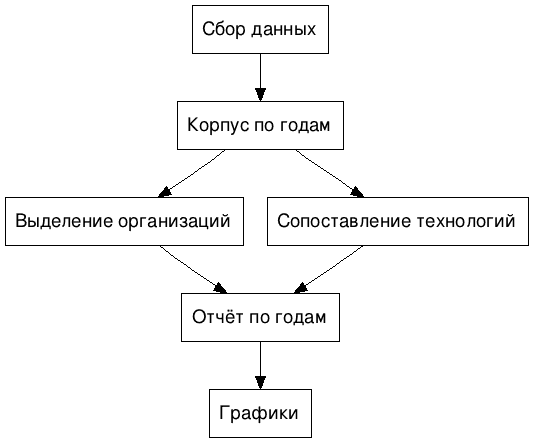
\includegraphics[height=3in]{pipeline.png}
\end{center}
\end{figure}
\end{frame}

%6. (Подходы к решению, решения, использованный инструментарий)

\begin{frame}\frametitle{Источники данных}

\begin{itemize}
    \item CrunchBase \item Habrahabr.ru \item Lenta.ru: <<Наука и техника>> \item Русскоязычная и англоязычная версии Википедии
\end{itemize}

\end{frame}

\begin{frame}\frametitle{Структура Википедии [1]}
Помимо статей, текстовых ссылок и заголовков, пользователями Википедии поддерживается <<дерево категорий>>

\begin{figure}[ht]
\begin{center}
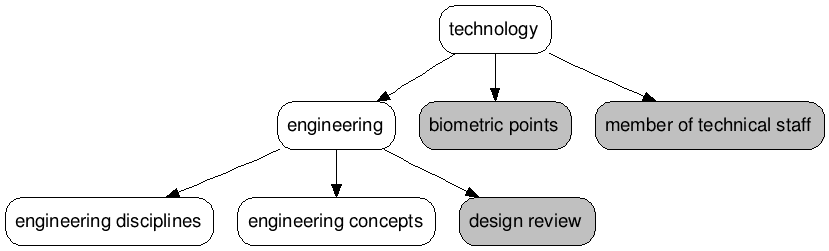
\includegraphics[width=4.5in]{chart_categories.png}
\end{center}
\end{figure}

\end{frame}
\begin{frame}\frametitle{Структура Википедии [2]}

\begin{figure}[ht]
\begin{center}
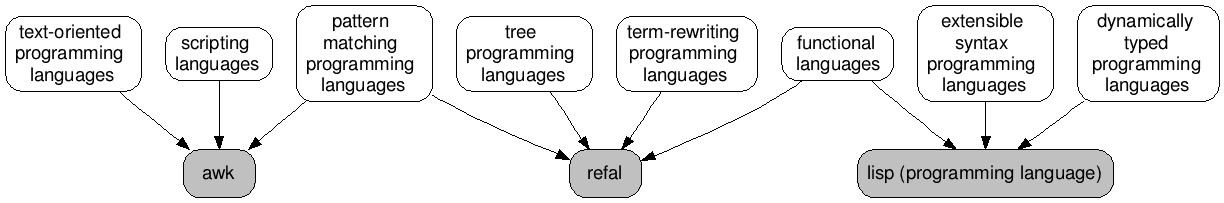
\includegraphics[width=4.5in]{chart_languages.png}
\end{center}
\end{figure}
\end{frame}


%7. Программный комплекс/программа: состав, архитектура, диаграммы
%классов, структура БД, фуекциональность, результаты работы и пр.

\begin{frame}\frametitle{Извлечение наименований организаций}
\begin{enumerate}
\item Токенизация
\item Стемминг
\item Поиск подстрок из сформированного списка предобработанных наименований организаций
\end{enumerate}
\end{frame}

\begin{frame}\frametitle{Извлечение технологических областей~[1]}
Первый этап --- предобработка
        \begin{enumerate}
		\item Токенизация
		\item Фильтрация по списку стоп-слов
		\item Фильтрация по списку слов, встречавшихся в текстах ссылок и заголовков Википедии
        \end{enumerate}

\end{frame}

\begin{frame}\frametitle{Извлечение технологических областей~[2]}

\begin{figure}[ht]
\begin{center}
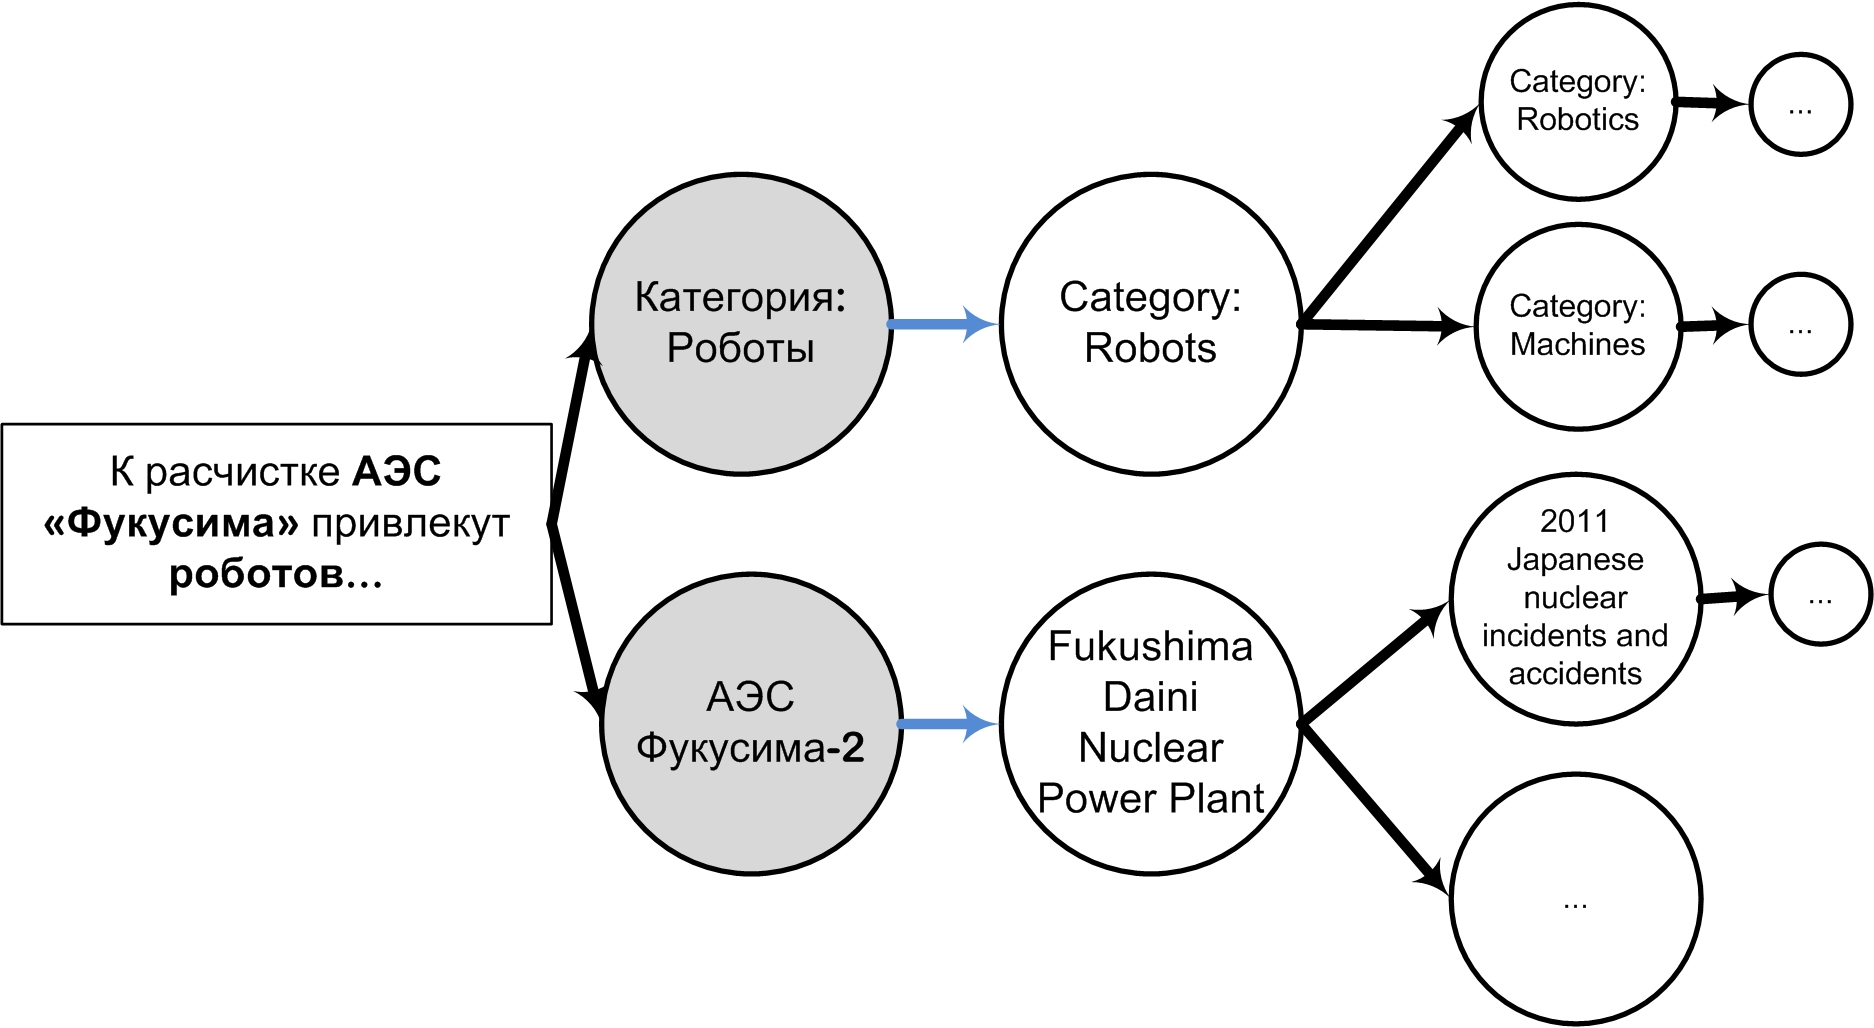
\includegraphics[width=4.5in]{Process.png}
\end{center}
\end{figure}

\end{frame}

\begin{frame}\frametitle{Пример результата работы}
\begin{figure}[ht]
\begin{center}
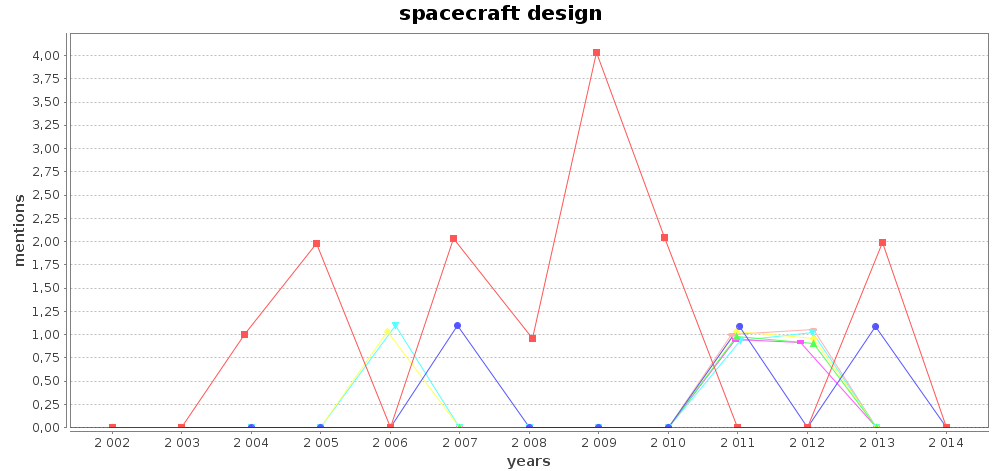
\includegraphics[width=4.5in]{space2.png}
\end{center}
\end{figure}
\begin{figure}[ht]
\begin{center}

\includegraphics[width=4.5in]{big_names.png}
\end{center}
\end{figure}
\end{frame}

\begin{frame}\frametitle{Использованный инструментарий}

%\begin{itemize}
%    \item Scala
%    \item Java
%    \item Python
%    \item WikiXMLJ
%    \item slf4j + logback
%    \item Apache Commons
%    \item Apache Lucene
%    \item Apache Maven
%\end{itemize}
(логотипы технологий нужны для того, чтобы размещать их на слайдах)
\end{frame}


\begin{frame}\frametitle{ЧСВ}
\begin{itemize}
    \item Подход представлен на <<СПИСОК-2014>>
    \item Доклад принят на <<НСМВ-2014>>
\end{itemize}
\end{frame}

\begin{frame}\frametitle{Благодарности}
	\begin{itemize}
		\item CSC, Яндекс, руководители практик
		\item<2> А ещё спасибо Papeeria за шаблон презентации
	\end{itemize}
\end{frame}

%10. Повтор титульного слайда

{
\title{Матчинг + извлечение трендов}
\institute{Причастны: Яндекс, HP Labs}
\setbeamertemplate{navigation symbols}{} 
\frame{\titlepage\label{lastframe}}
}

%{
%\setbeamertemplate{navigation symbols}{} 
%\begin{frame}\frametitle{Выбор значимых технологических областей}
%$$\textrm{keyphraseness}=\frac{\textrm{Freq}_{link}}{\textrm{Freq}_{body}}$$
%\end{frame}
%}
\end{document}
